\documentclass[a4paper]{ctexart}
\usepackage{amsmath}
\usepackage{graphicx}
\usepackage{hyperref}
\usepackage{float}
\usepackage{geometry}
\title{光衍射的定量研究}
\author{陈启钰\,\,2300011447}
\date{\today}
\begin{document}
	\maketitle
	\tableofcontents
	\newpage
	\section{单缝缝宽的测量}
	单缝衍射测量得到的光强分布如图所示
	\begin{figure}[H]
		\centering
		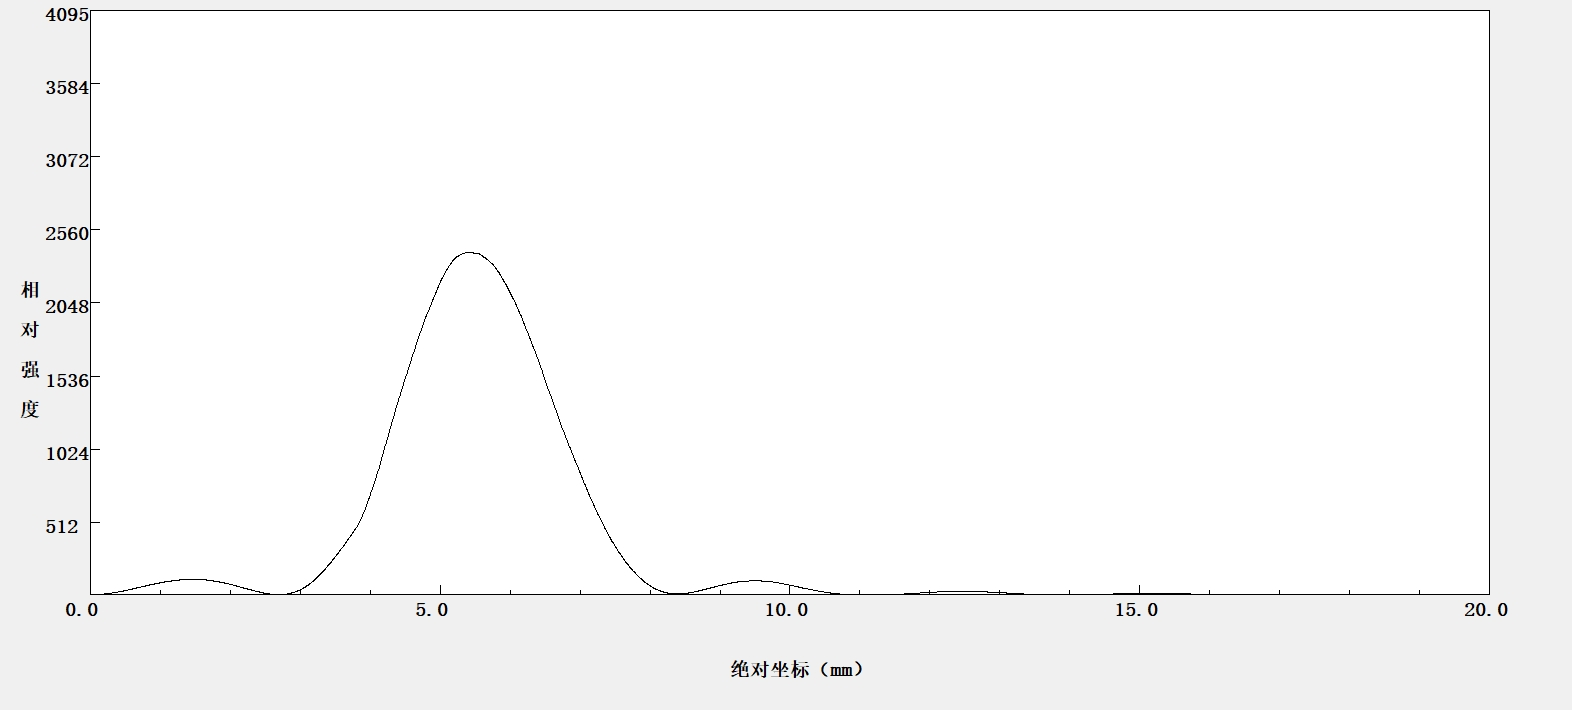
\includegraphics[width=10cm]{danfeng.jpg}
		\caption{单缝衍射光强分布}
	\end{figure}
	\begin{table}[H]
		\begin{center}
			\caption{单缝衍射主极大和次极大测量值}
			\begin{tabular}{c|ccc}
				$i$&1&2&3\\
				\hline
				$x_i/\mathrm{mm}$&1.400&5.405&9.470\\
				\hline
				相对光强$I_i$&113&2401&103
			\end{tabular}
		\end{center}
	\end{table}
	可以验证
	\begin{align}
		\frac{|I_1-I_3|}{\frac{I_1+I_3}{2}}=9.26\%<10\%
	\end{align}
	以及
	\begin{align}
		\frac{\frac{I_1+I_3}{2}}{I_2}=4.5\%
	\end{align}
	与$4.7\%$的相对差距小于$5\%$,所以该次测量得到的光强分布可以认为是关于主极强是对称的,可以进行缝宽的计算。
	衍射屏到光强接收器的距离
	\begin{align}
		z=779.0\mathrm{mm}
	\end{align}
	屏上次极强到主极强的距离
	\begin{align}
		\Delta x=\frac{x_3-x_1}{2}=4.035\mathrm{mm}
	\end{align}
	根据缝宽的计算公式可得
	\begin{align}
		b=\frac{1.43\lambda z}{\Delta x}=174.7\mathrm{\mu m}
	\end{align}
	与标准缝宽$b_0=175\mathrm{\mu m}$的相对差距
	\begin{align}
		B=0.17\%
	\end{align}
	可见这个差距是相当小的,也就是说测得的结果很准确。
	\section{三缝衍射的缝宽及缝间距测量}
	三缝得到的光强分布如图所示
	\begin{figure}[H]
		\centering
		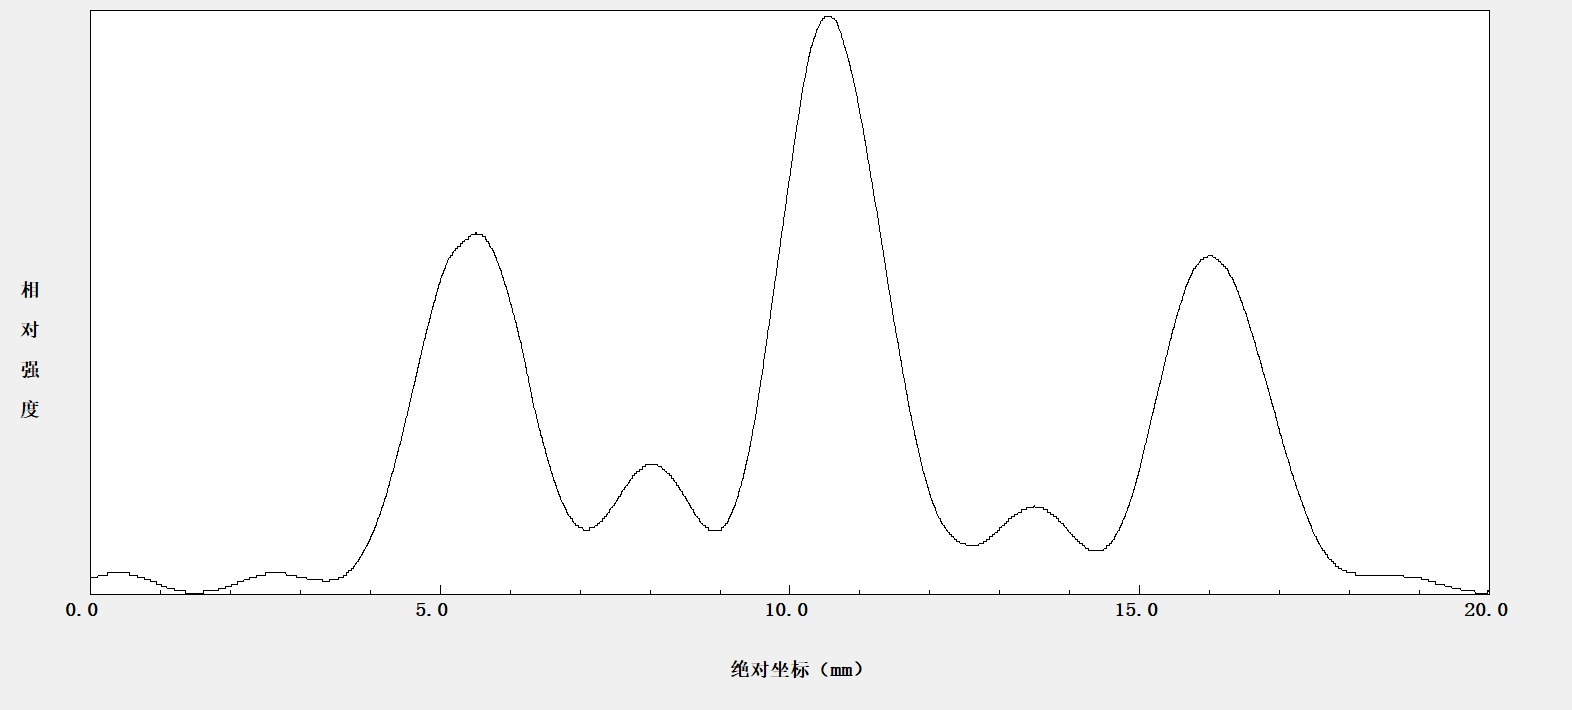
\includegraphics[width=10cm]{sanfeng.jpg}
		\caption{三缝衍射光强分布}
	\end{figure}
	一些关键数据点的测量结果如下(包括主极强,两个次极强以及两个极小)
	\begin{table}[H]
		\label{table}
		\begin{center}
			\caption{三缝衍射数据记录表}
			\begin{tabular}{c|ccccc}
				$i$&1&2&3&4&5\\
				\hline
				$x_i/\mathrm{mm}$&5.505&10.710&15.980&8.940&12.651\\
				\hline
				相对光强$I_i$&161&257&151&29&22
			\end{tabular}
		\end{center}
	\end{table}
	先算缝间距,第一个极小点到主峰的距离
	\begin{align}
		\Delta x=\frac{x_4+x_5}{2}=1.856\mathrm{\mu m}
	\end{align}
	缝间距
	\begin{align}
		d=\frac{1}{3}\frac{\lambda z}{\Delta x}=88.53\mathrm{\mu m}
	\end{align}
	与标准值$d_0=90\mathrm{\mu m}$差距
	\begin{align}
		B_d=1.6\%
	\end{align}
	再求缝宽,由光强分布公式可知,主峰和次极大的光强之比应为
	\begin{align}
		\left(\frac{\sin {\alpha}}{\alpha}\right)^2=\frac{\frac{I_1+I_3}{2}}{I_2}=0.607
	\end{align}
	式中
	\begin{align}
		\alpha=\frac{\pi b \Delta x/z}{\lambda}
	\end{align}
	解得
	\begin{align}
		\alpha=1.193
	\end{align}
	而
	\begin{align}
		\Delta x=\frac{x_3-x_1}{2}=5.238\mathrm{mm}
	\end{align}
	从而可计算缝宽
	\begin{align}
		b=1.193\frac{\lambda z}{\pi \Delta x}=35.74\mathrm{\mu m}
	\end{align}
	与标准值$b_0=40\mathrm{\mu m}$的差距
	\begin{align}
		B_b=11\%
	\end{align}
	这里只能说缝宽的测量结果是合理的,不能说是准确的。下面略微进行一些分析。\\
	根据表\ref{table}可以看出,三缝衍射的光强分布图对称性不是特别好,主峰两边的极大值和极小值都有一些偏移,这可能造成了一定的误差。还有我们在解$\alpha$时,解方程的过程可能会放大光强测量的误差,从而导致$\alpha$的误差相对变大。但总体来说,这个结果还是可以接受的。
	\section{其它形状的衍射图案}
	\subsection{单方孔衍射}
	\begin{figure}[H]
		\centering
		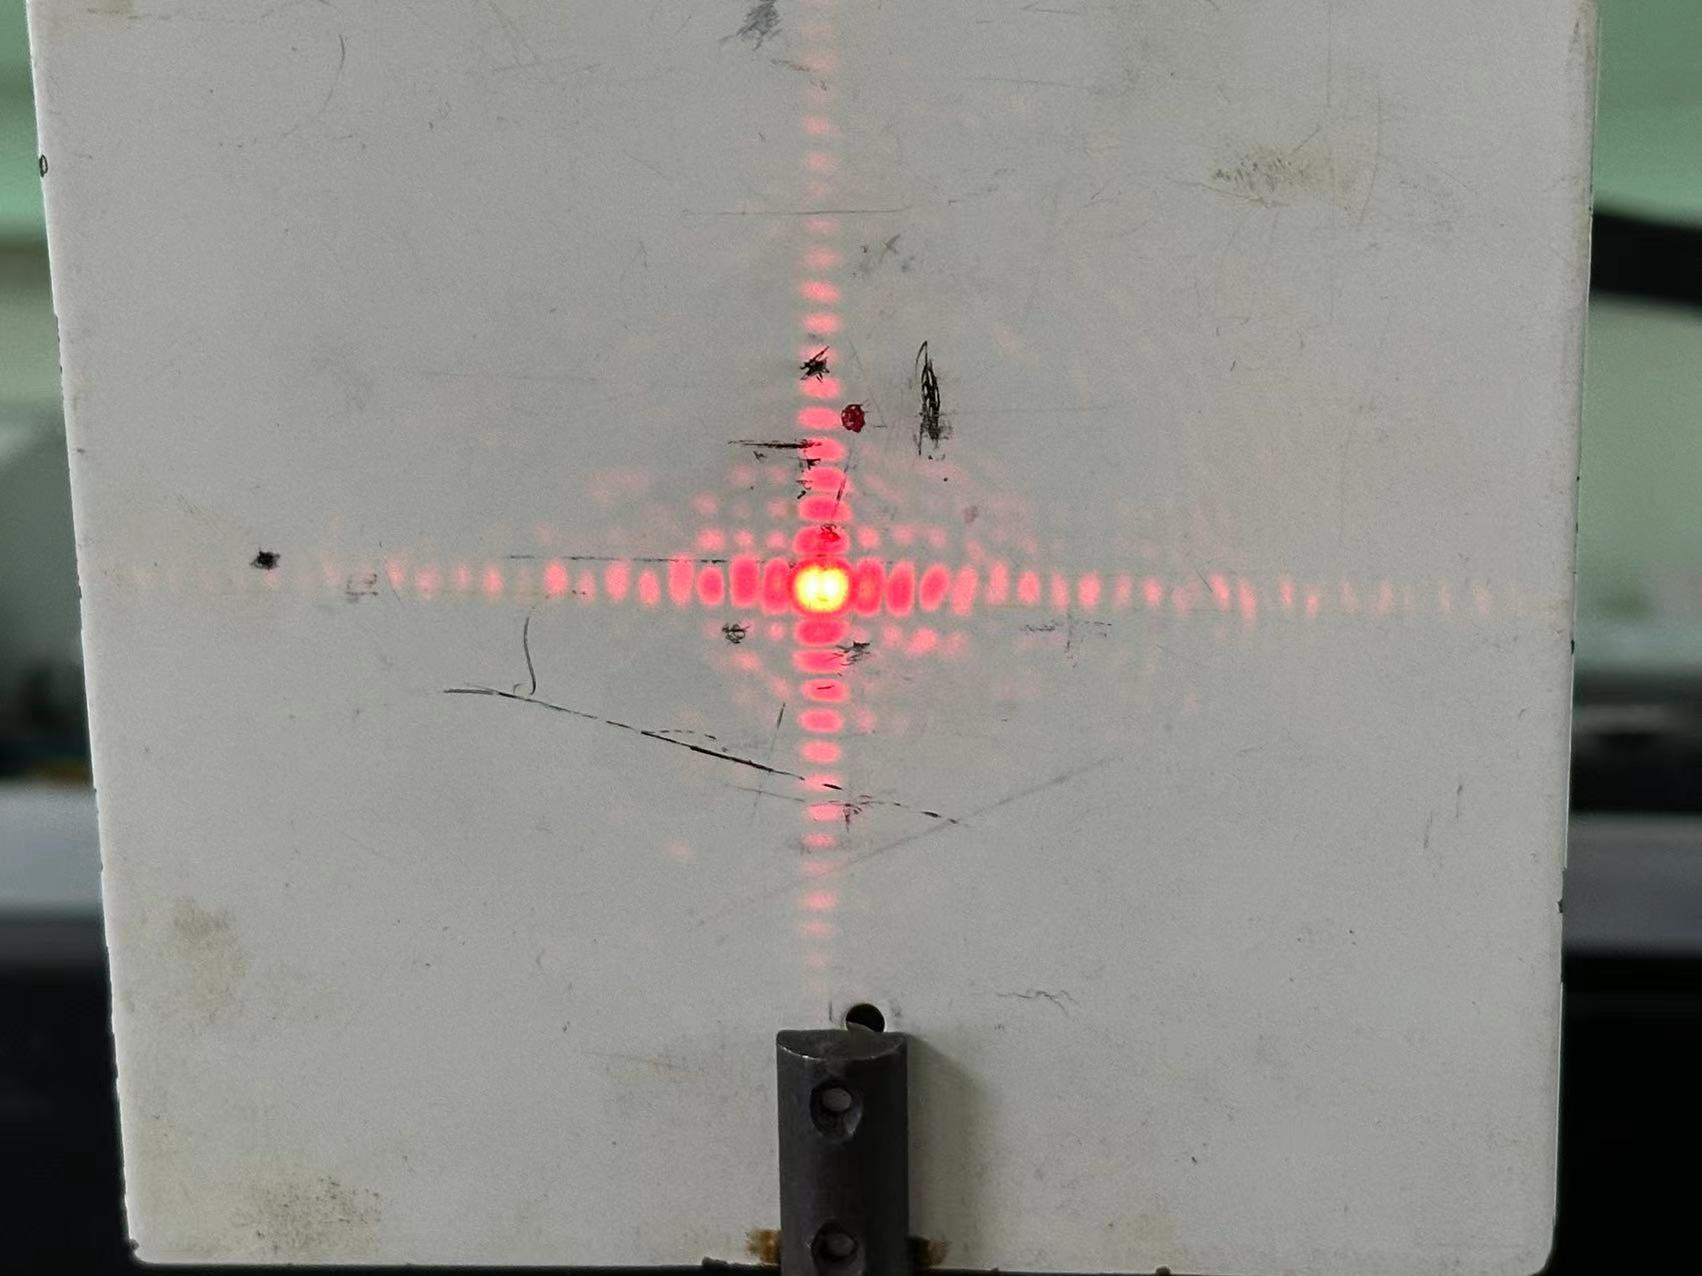
\includegraphics[width=6cm]{1.jpg}
		\caption{单方孔衍射图案}
	\end{figure}
	\subsection{双方孔衍射}
	\begin{figure}[H]
		\centering
		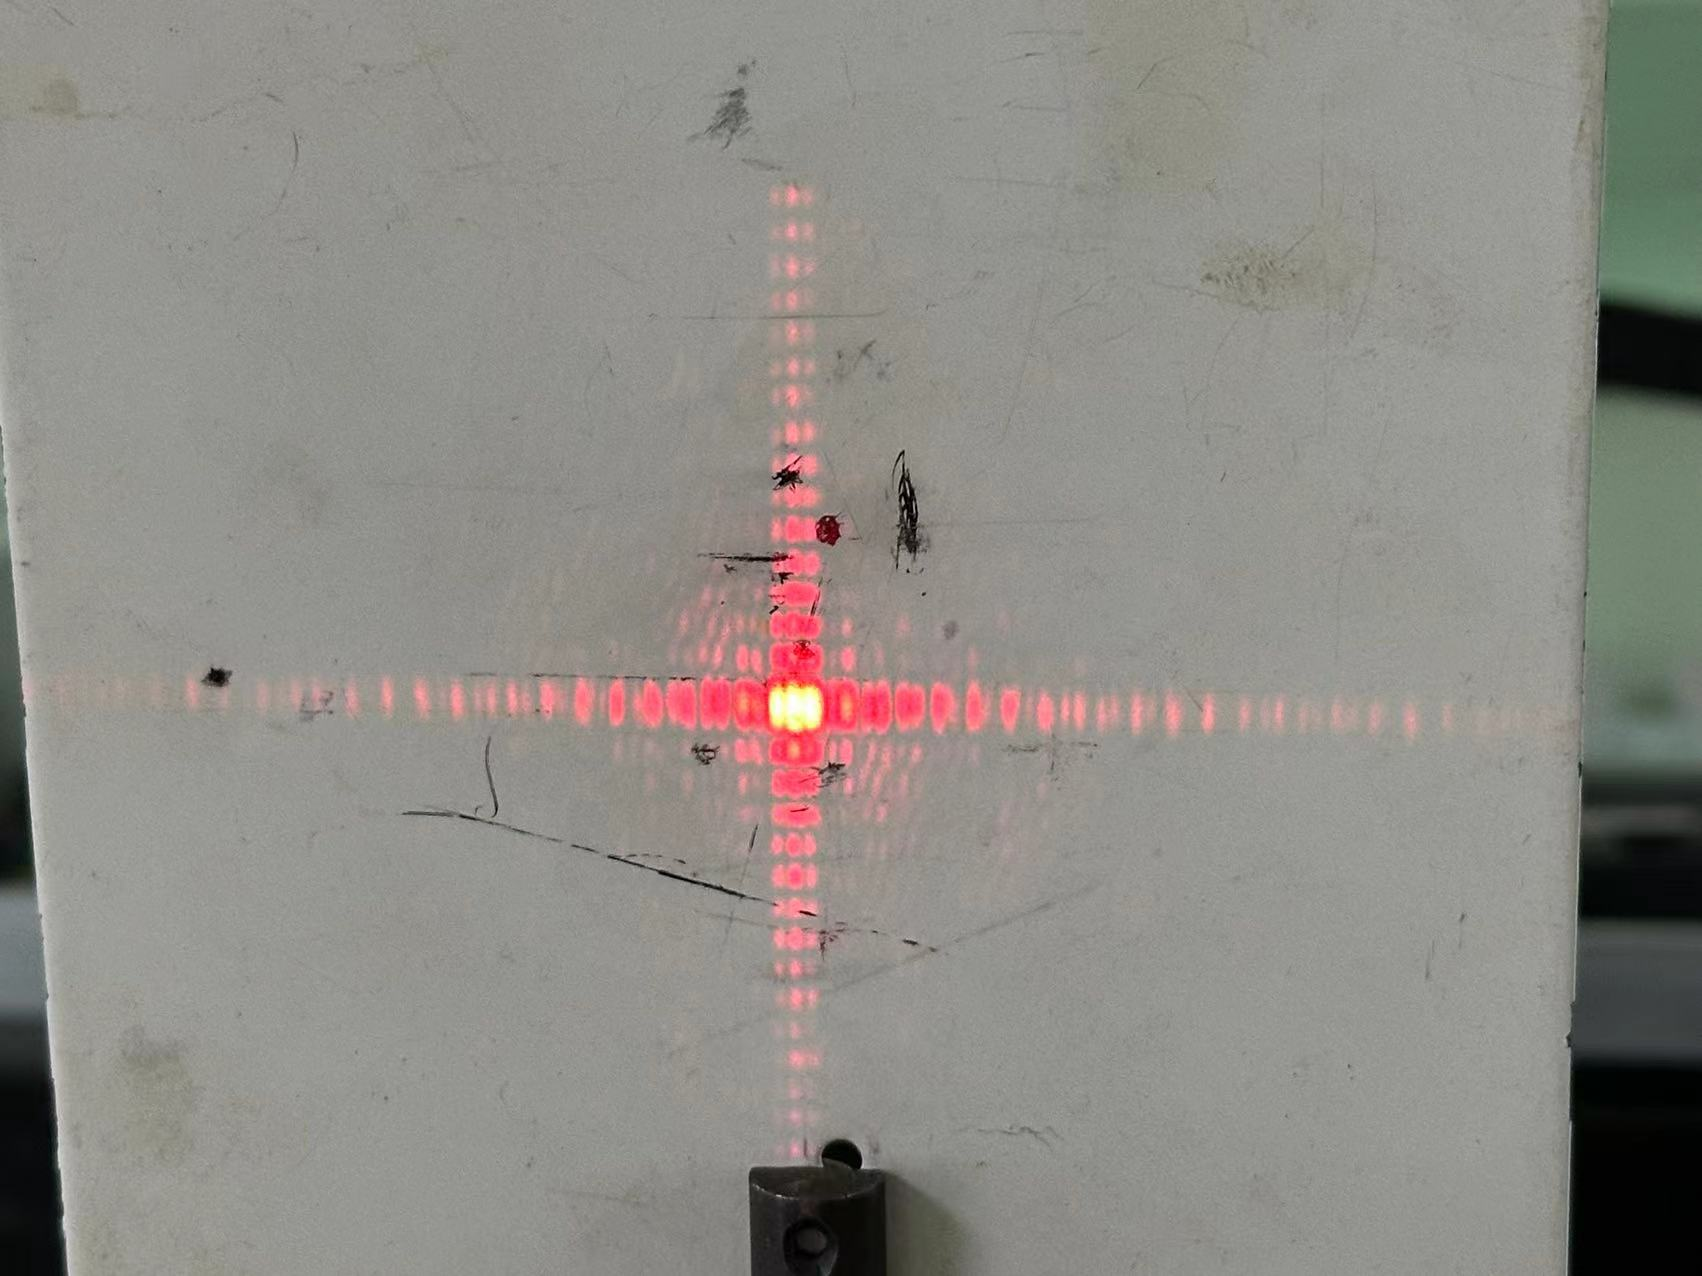
\includegraphics[width=6cm]{2.jpg}
		\caption{双方孔衍射图案}
	\end{figure}
	\subsection{方孔方阵衍射}
	\begin{figure}[H]
		\centering
		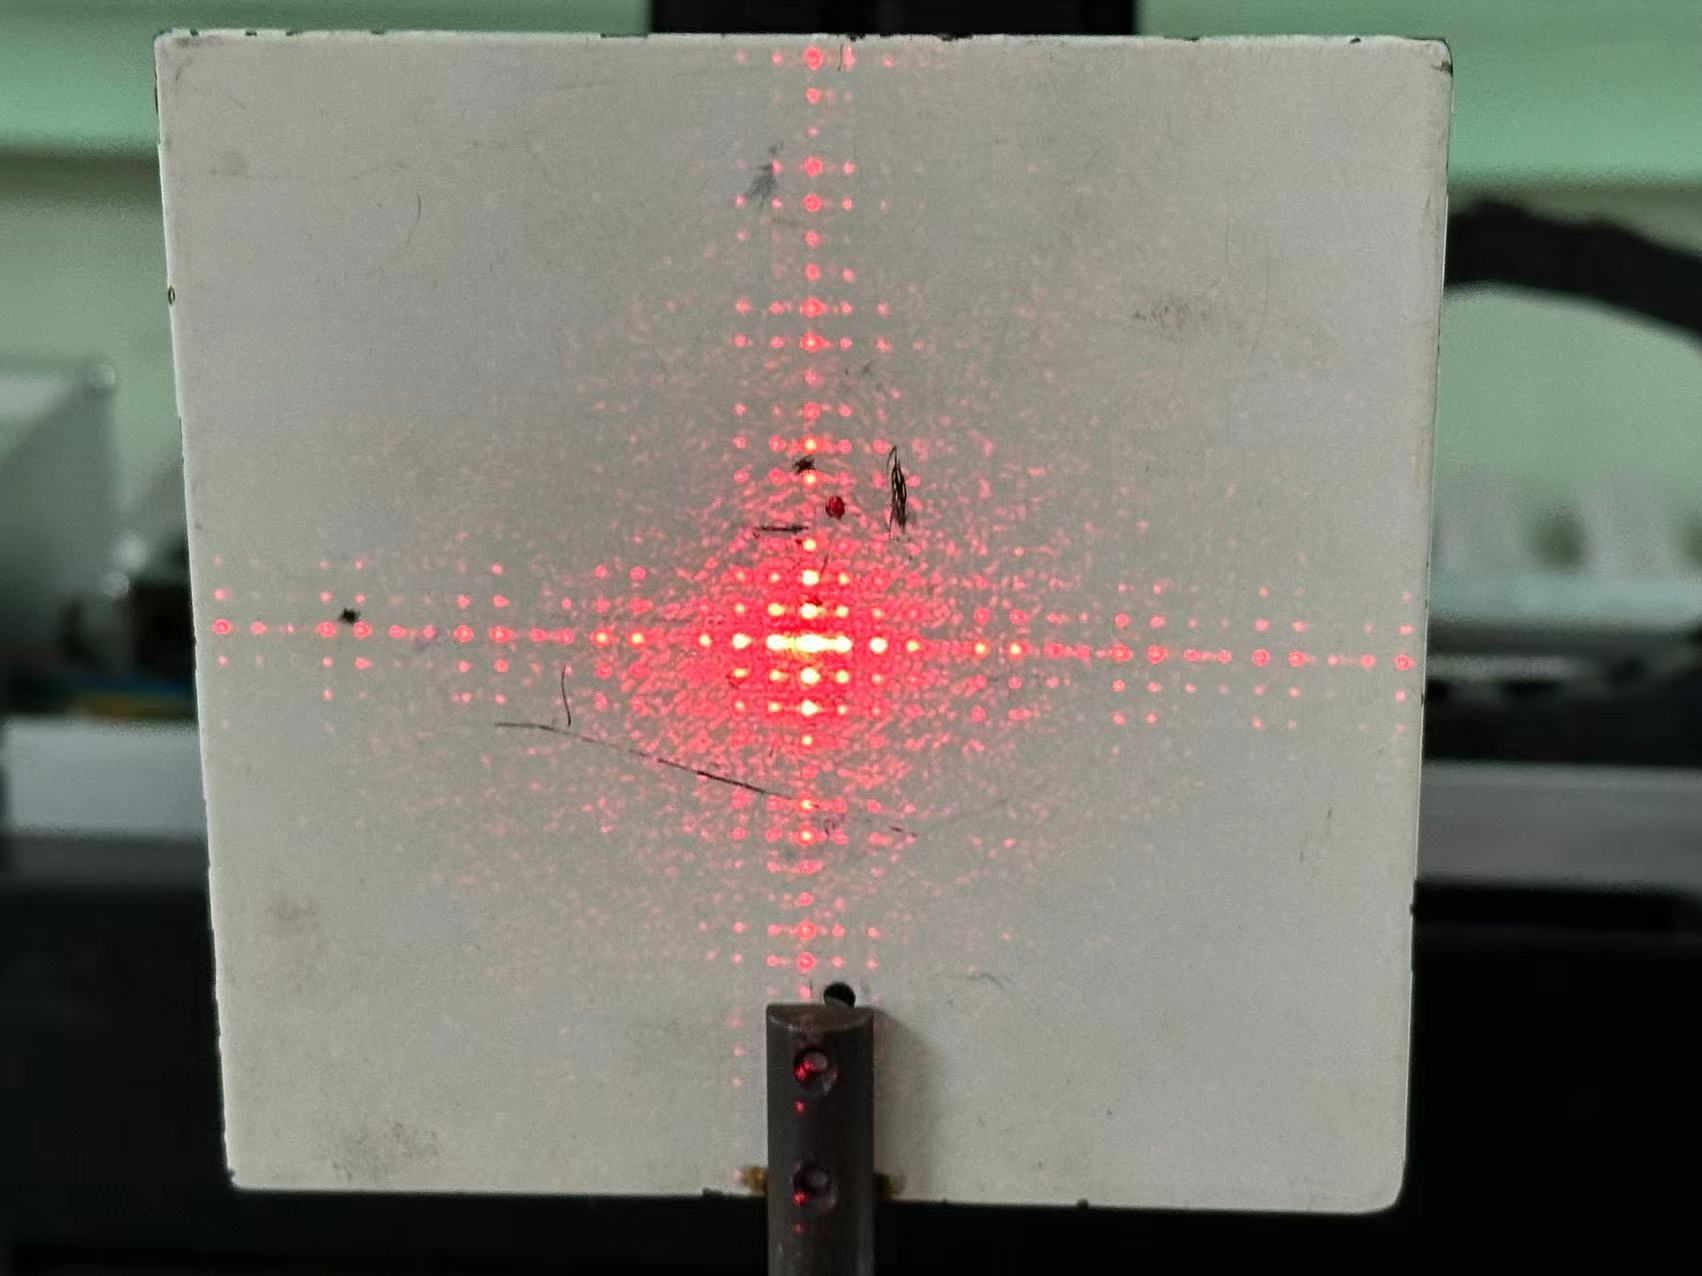
\includegraphics[width=6cm]{3.jpg}
		\caption{方孔方阵衍射图案}
	\end{figure}
	\subsection{方孔密排衍射}
	\begin{figure}[H]
		\centering
		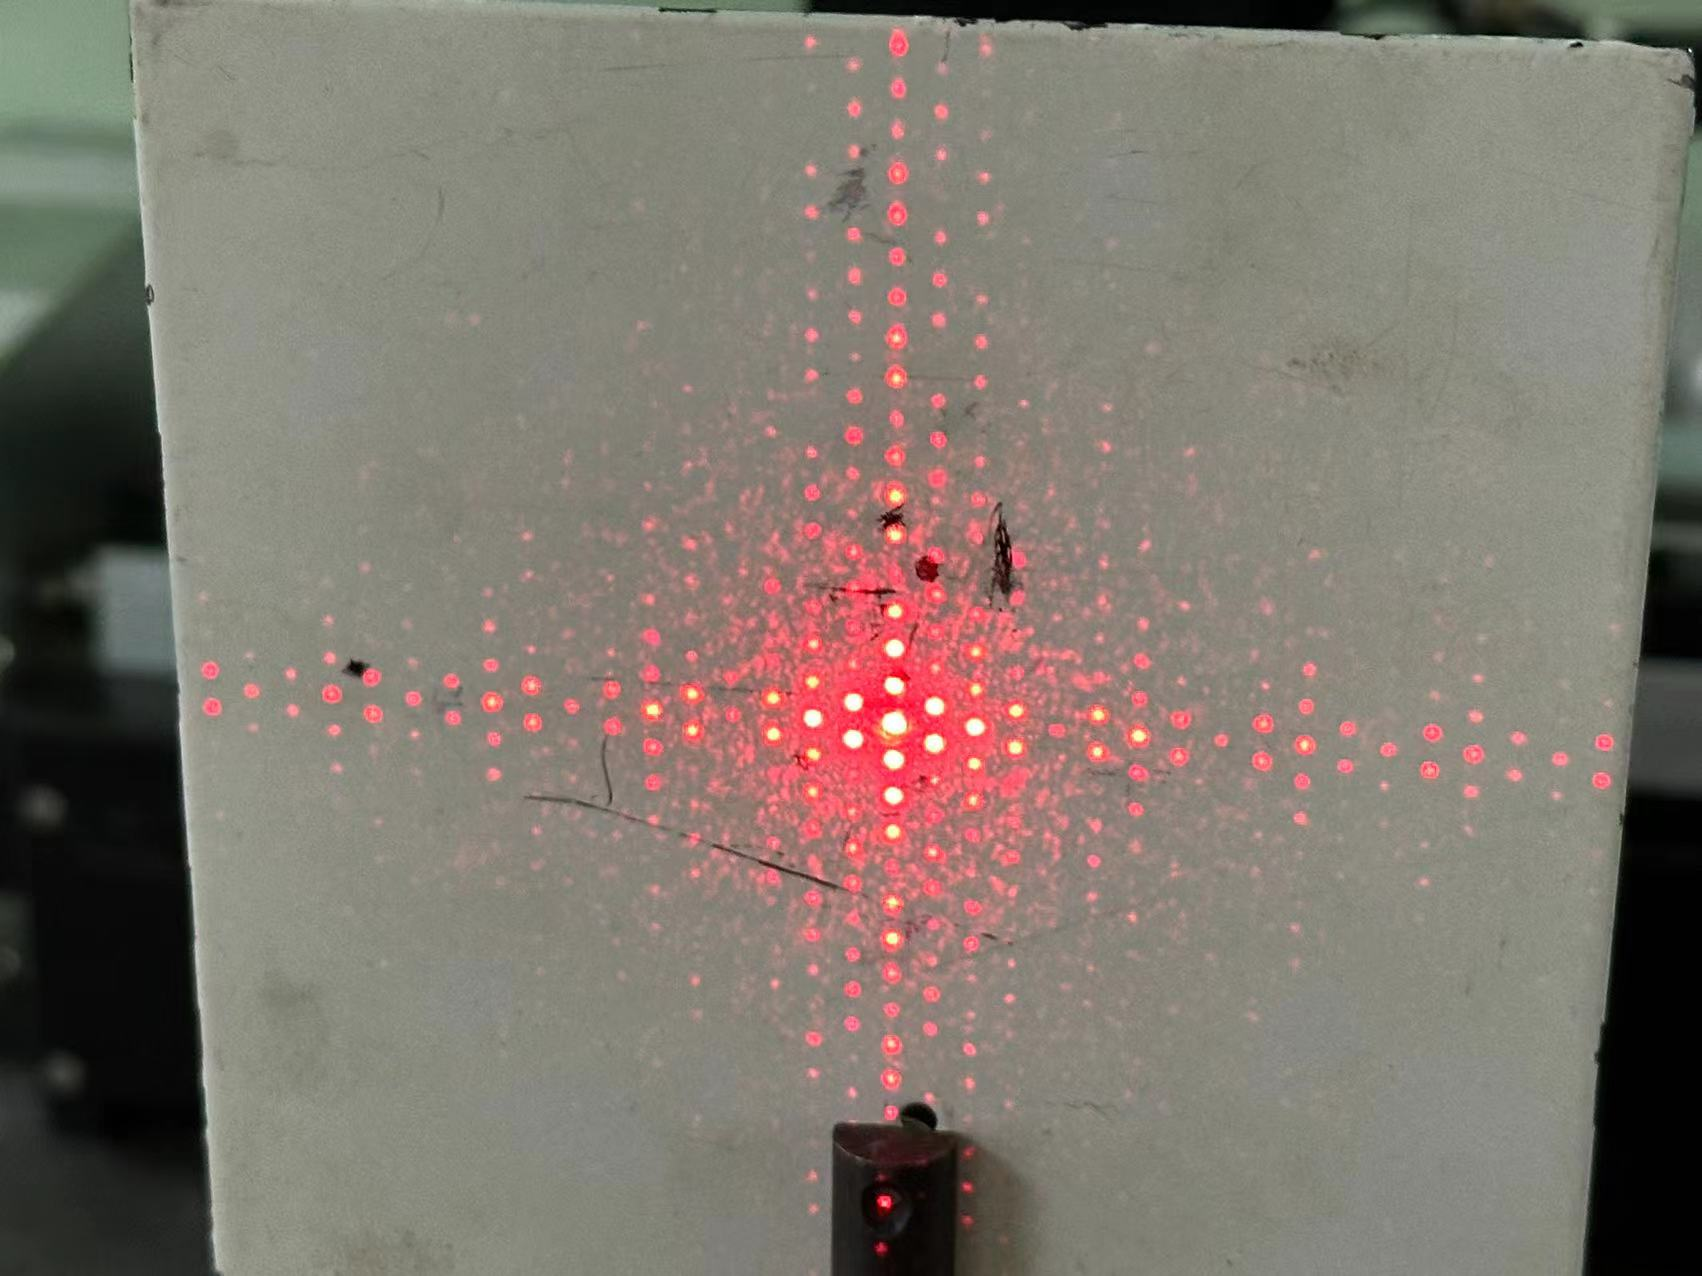
\includegraphics[width=6cm]{4.jpg}
		\caption{方孔密排衍射图案}
	\end{figure}
	\subsection{单圆孔衍射}
	\begin{figure}[H]
		\centering
		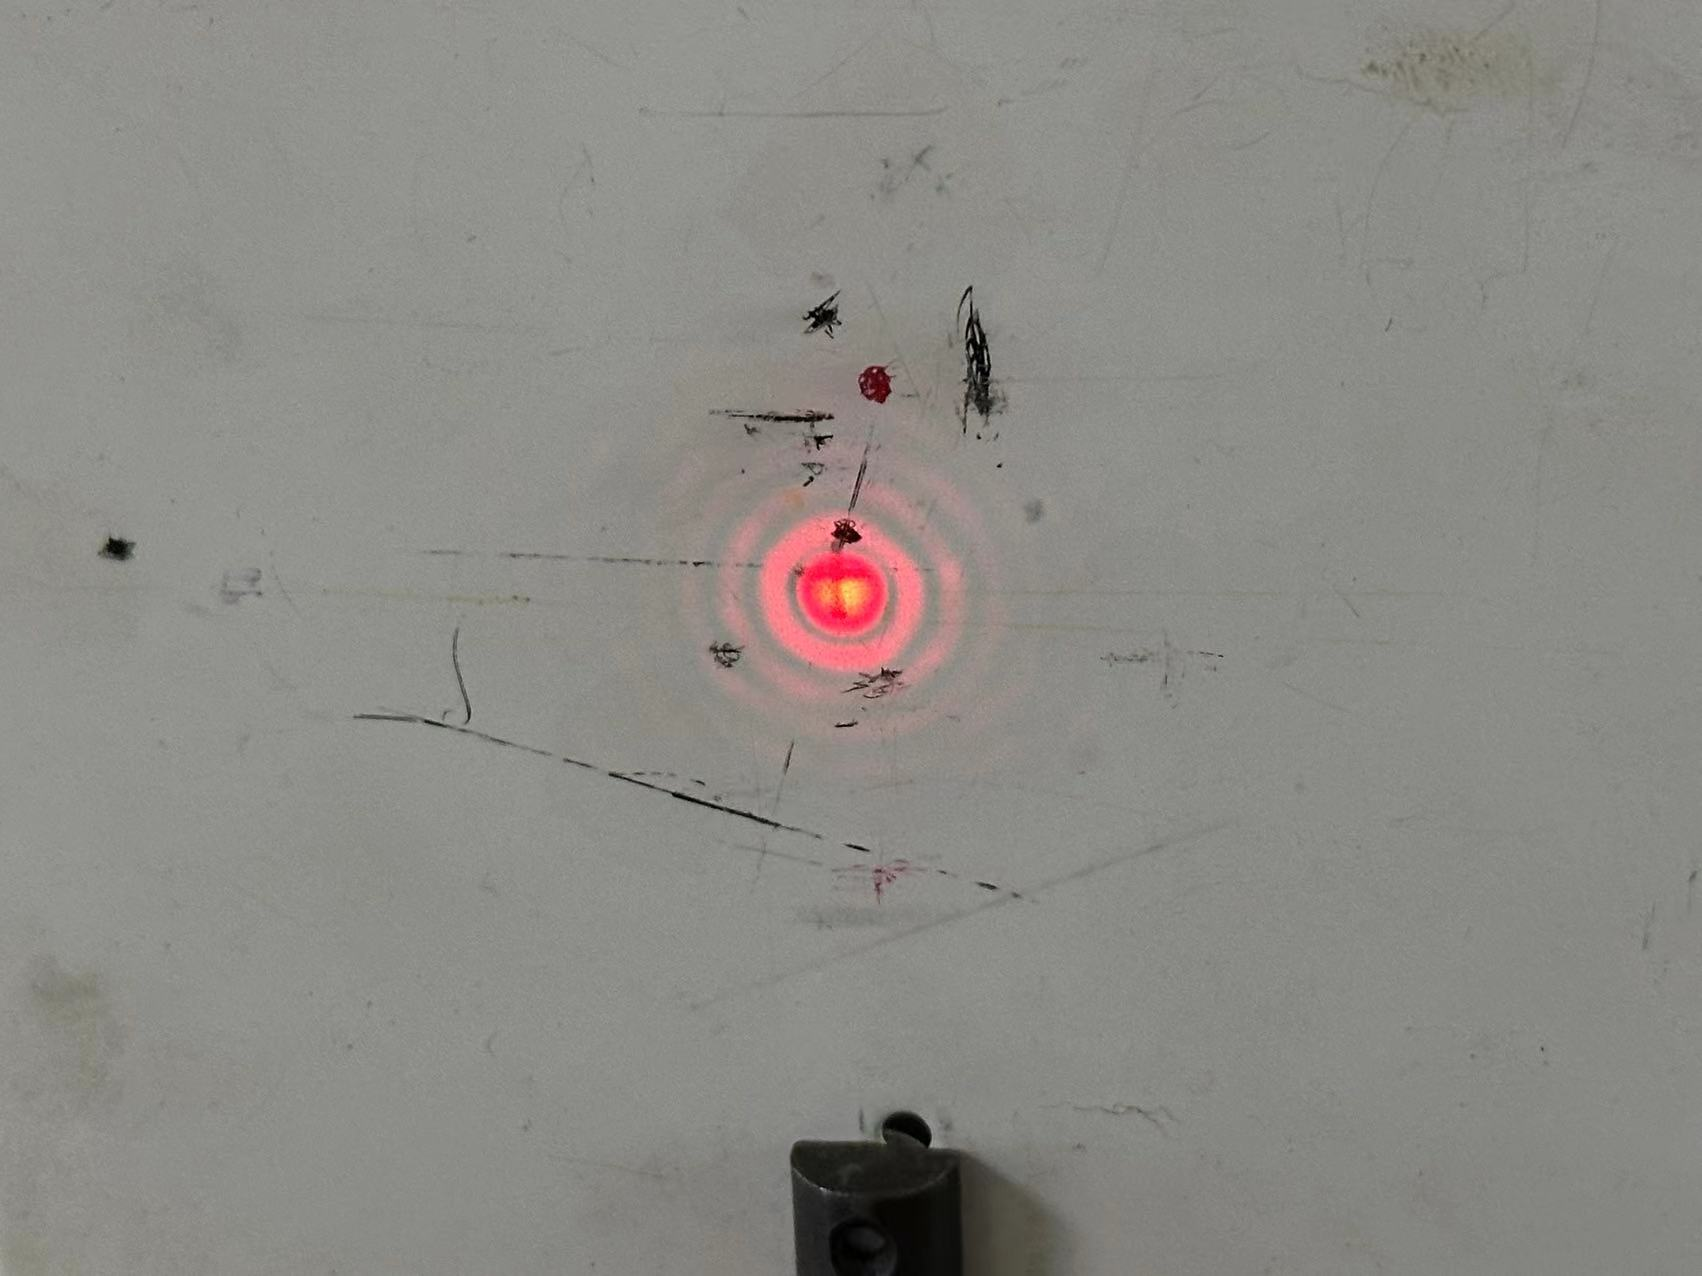
\includegraphics[width=6cm]{5.jpg}
		\caption{单圆孔衍射图案}
	\end{figure}
	\subsection{双圆孔衍射}
	\begin{figure}[H]
		\centering
		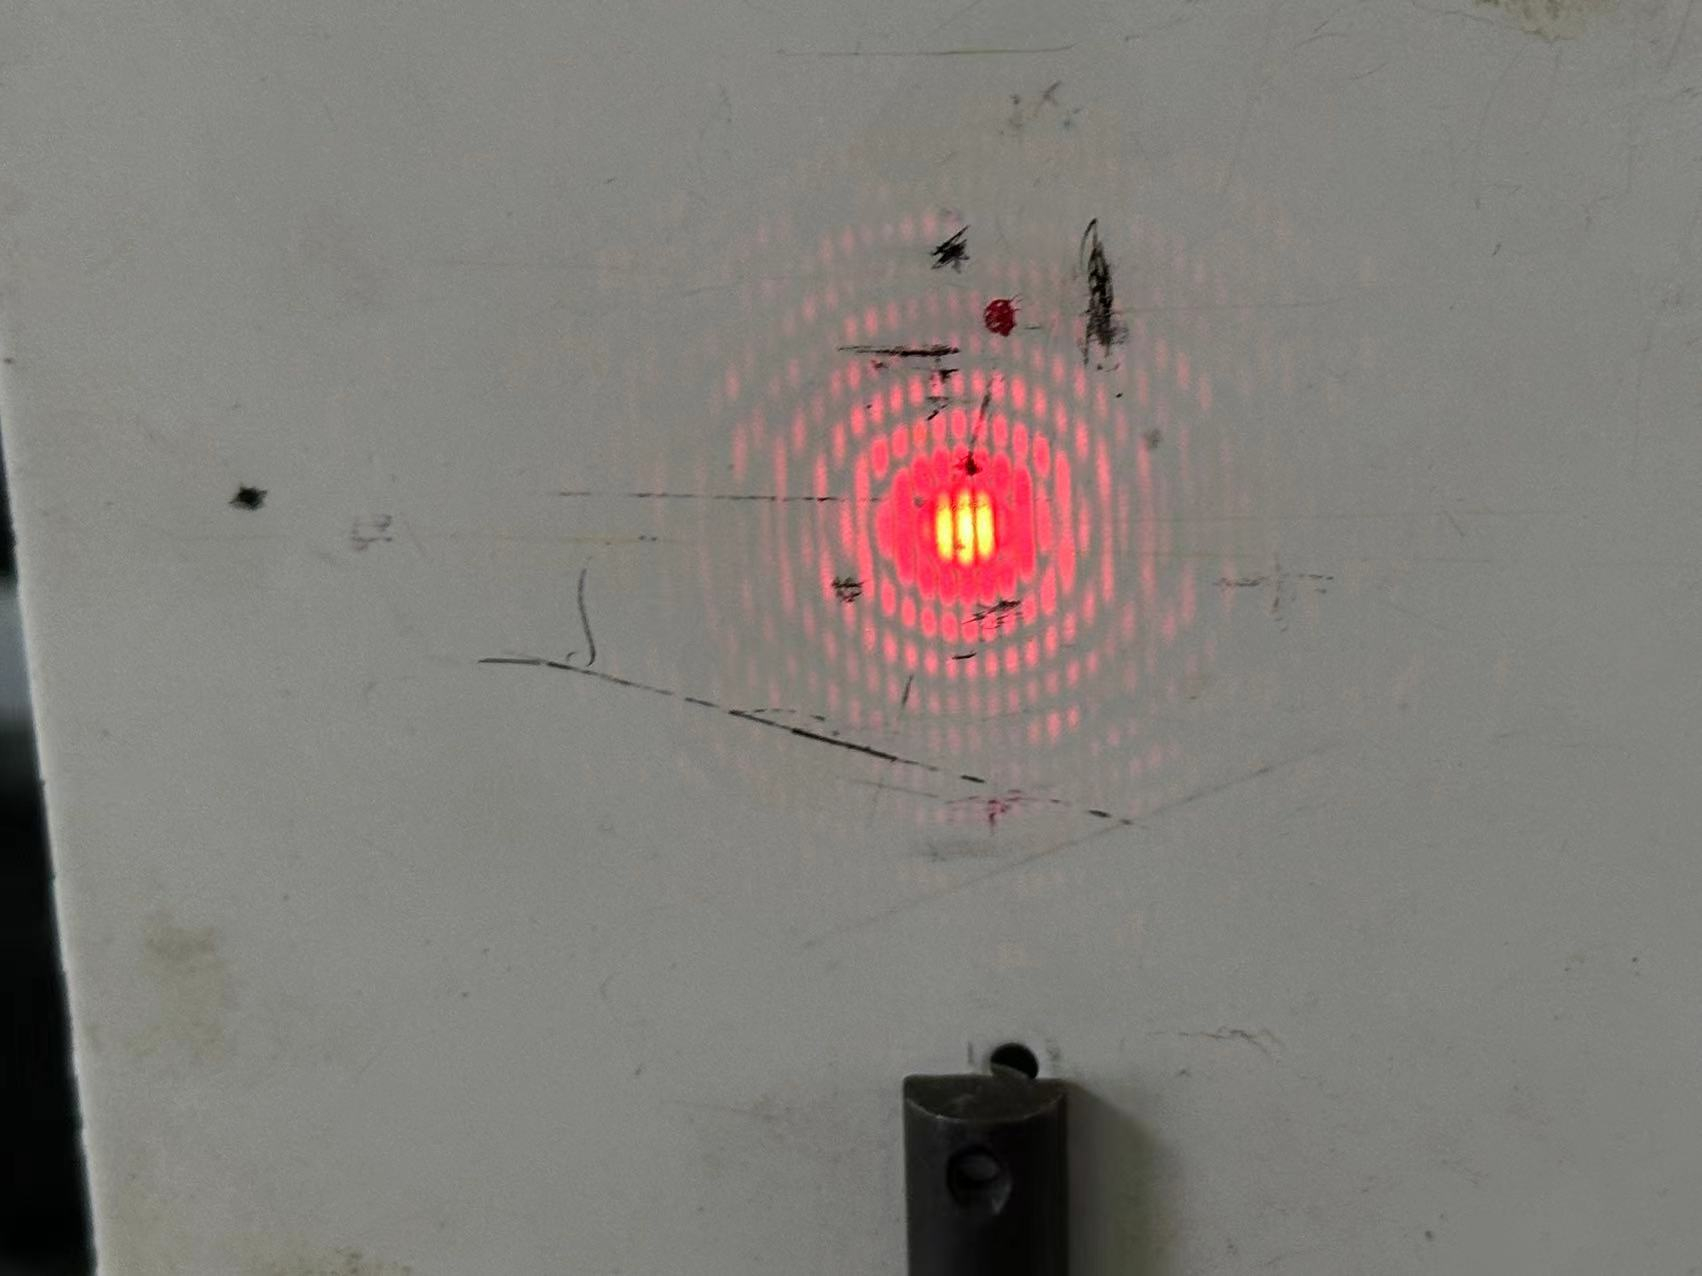
\includegraphics[width=6cm]{6.jpg}
		\caption{双圆孔衍射图案}
	\end{figure}
	\subsection{圆孔方阵衍射}
	\begin{figure}[H]
		\centering
		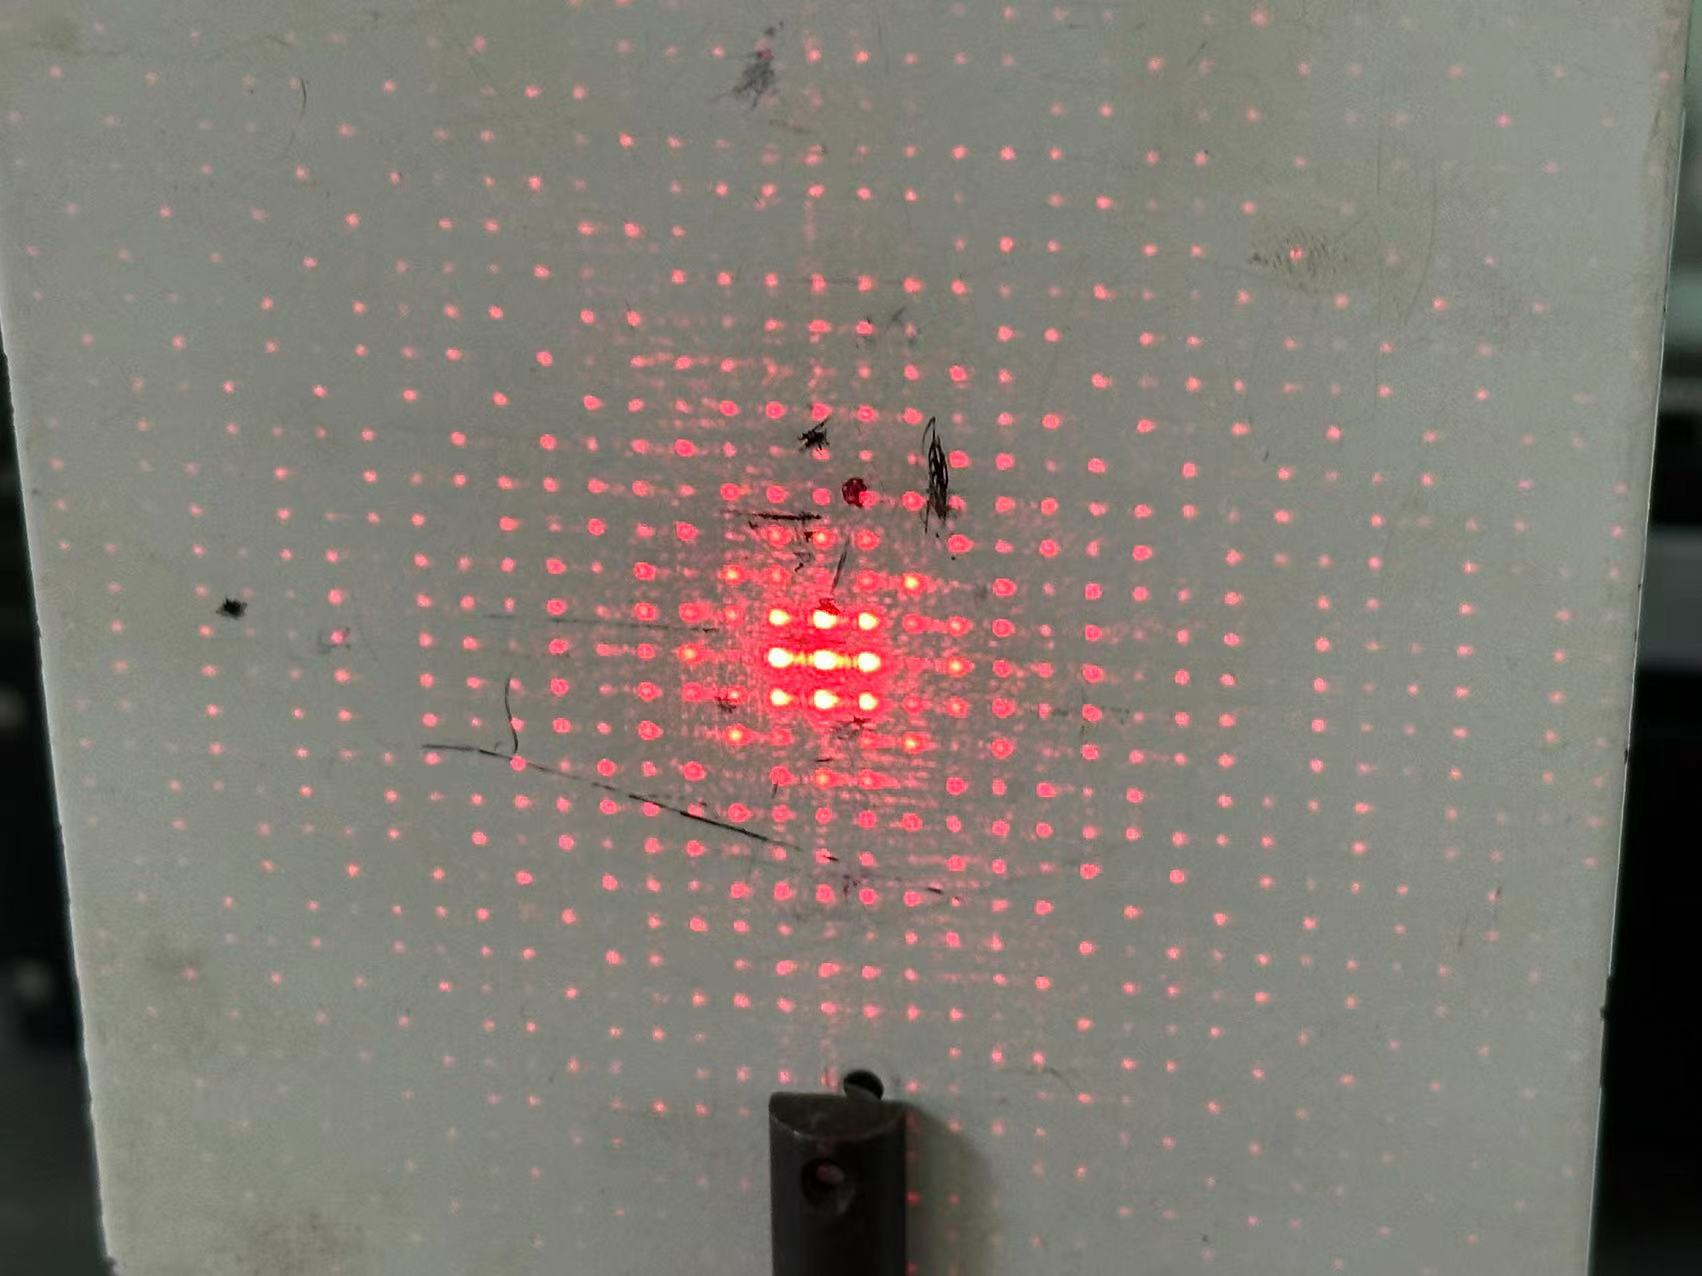
\includegraphics[width=6cm]{7.jpg}
		\caption{圆孔方阵衍射图案}
	\end{figure}
	\subsection{圆孔密排衍射}
	\begin{figure}[H]
		\centering
		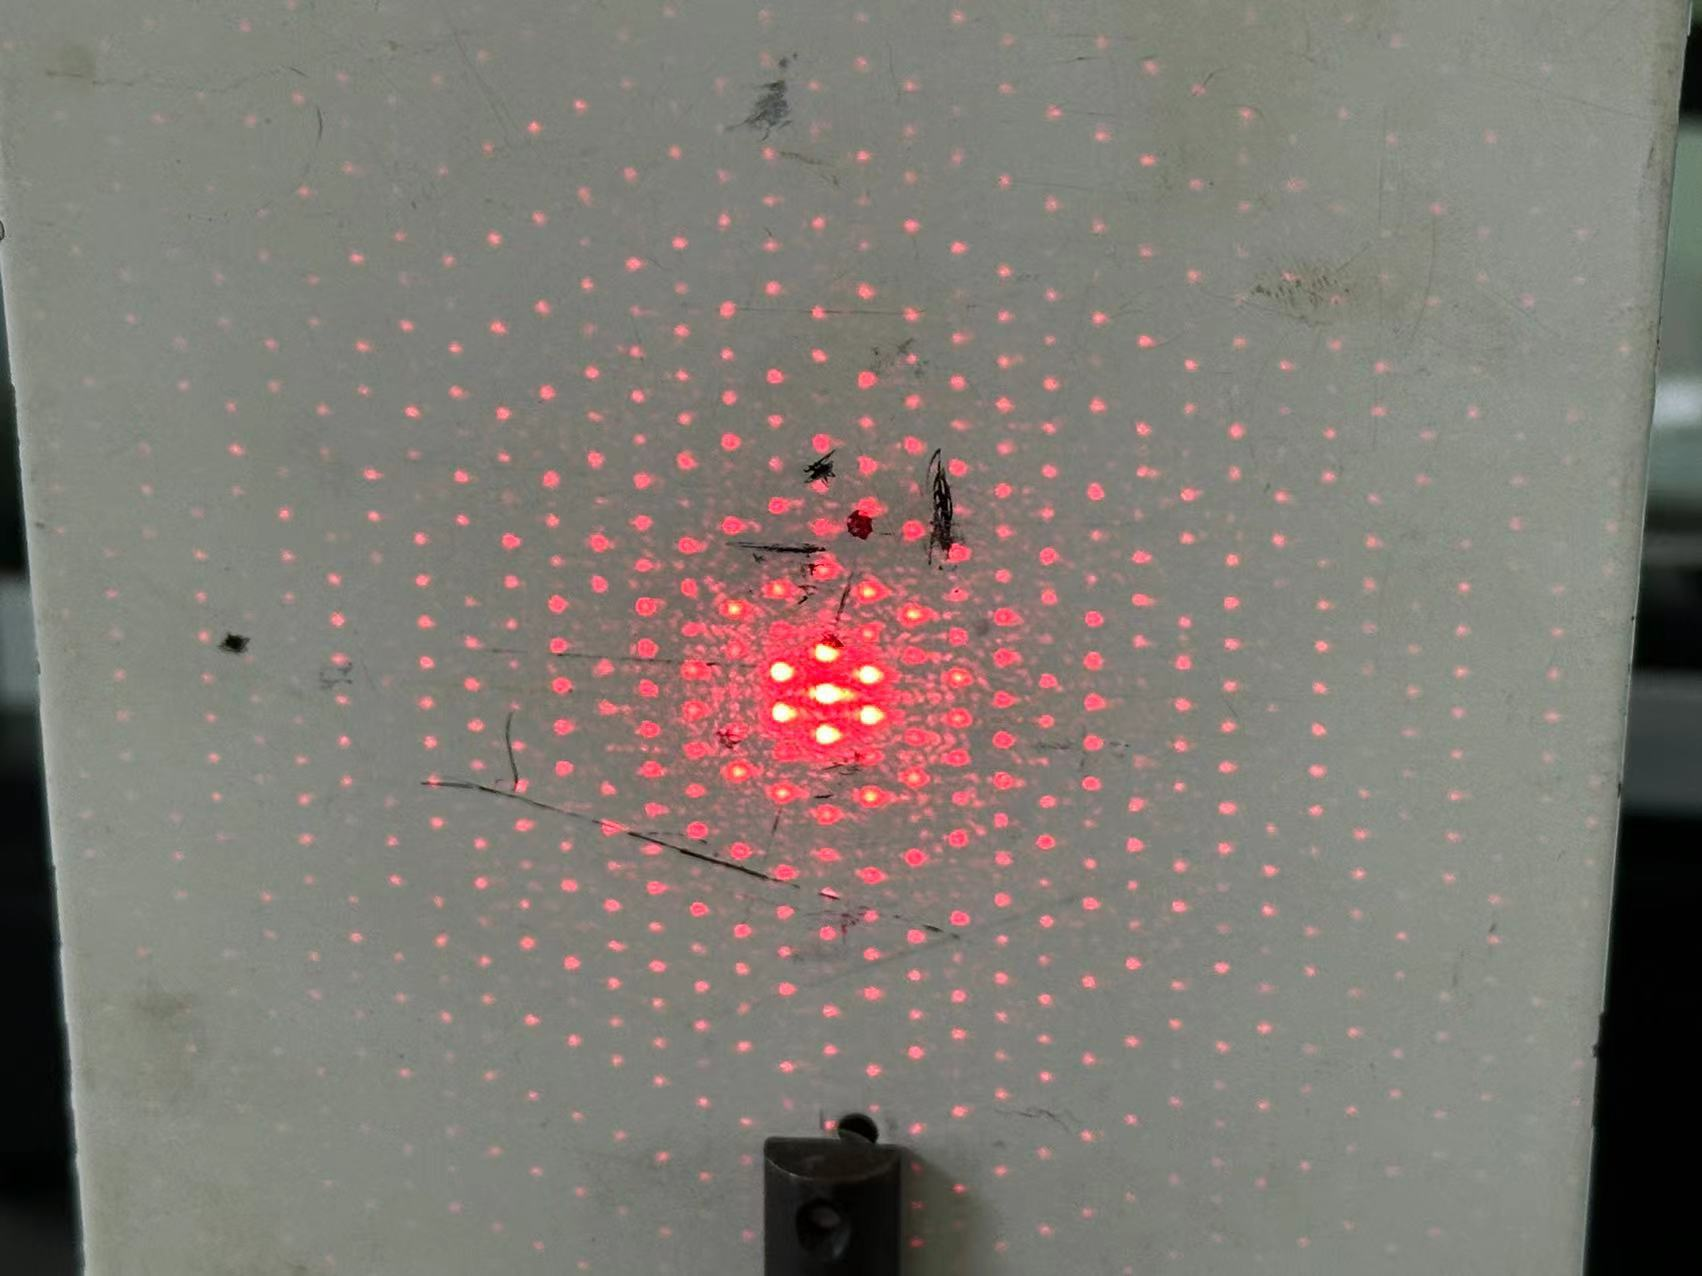
\includegraphics[width=6cm]{8.jpg}
		\caption{圆孔密排衍射图案}
	\end{figure}
	\subsection{等边三角形衍射}
	\begin{figure}[H]
		\centering
		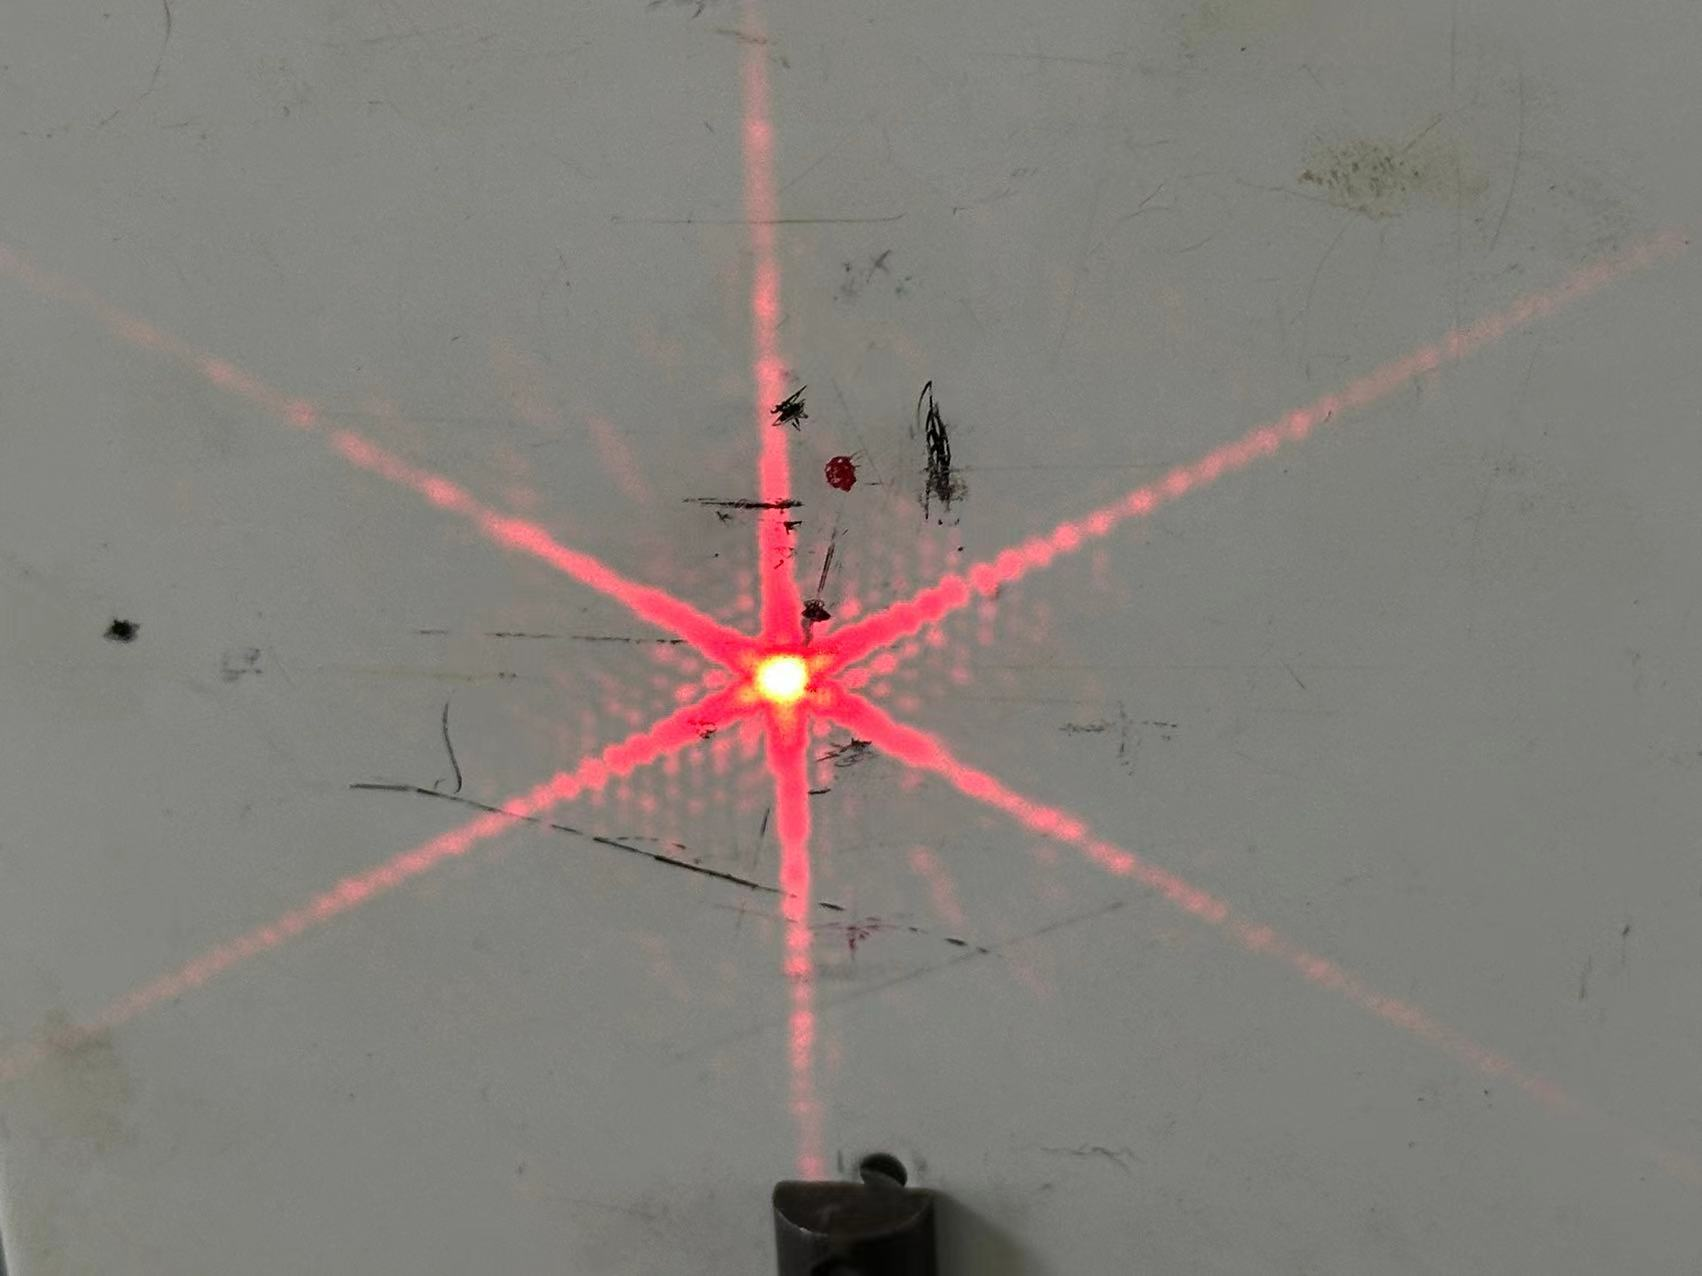
\includegraphics[width=6cm]{9.jpg}
		\caption{等边三角形衍射图案}
	\end{figure}
	\subsection{等腰三角形衍射}
	\begin{figure}[H]
		\centering
		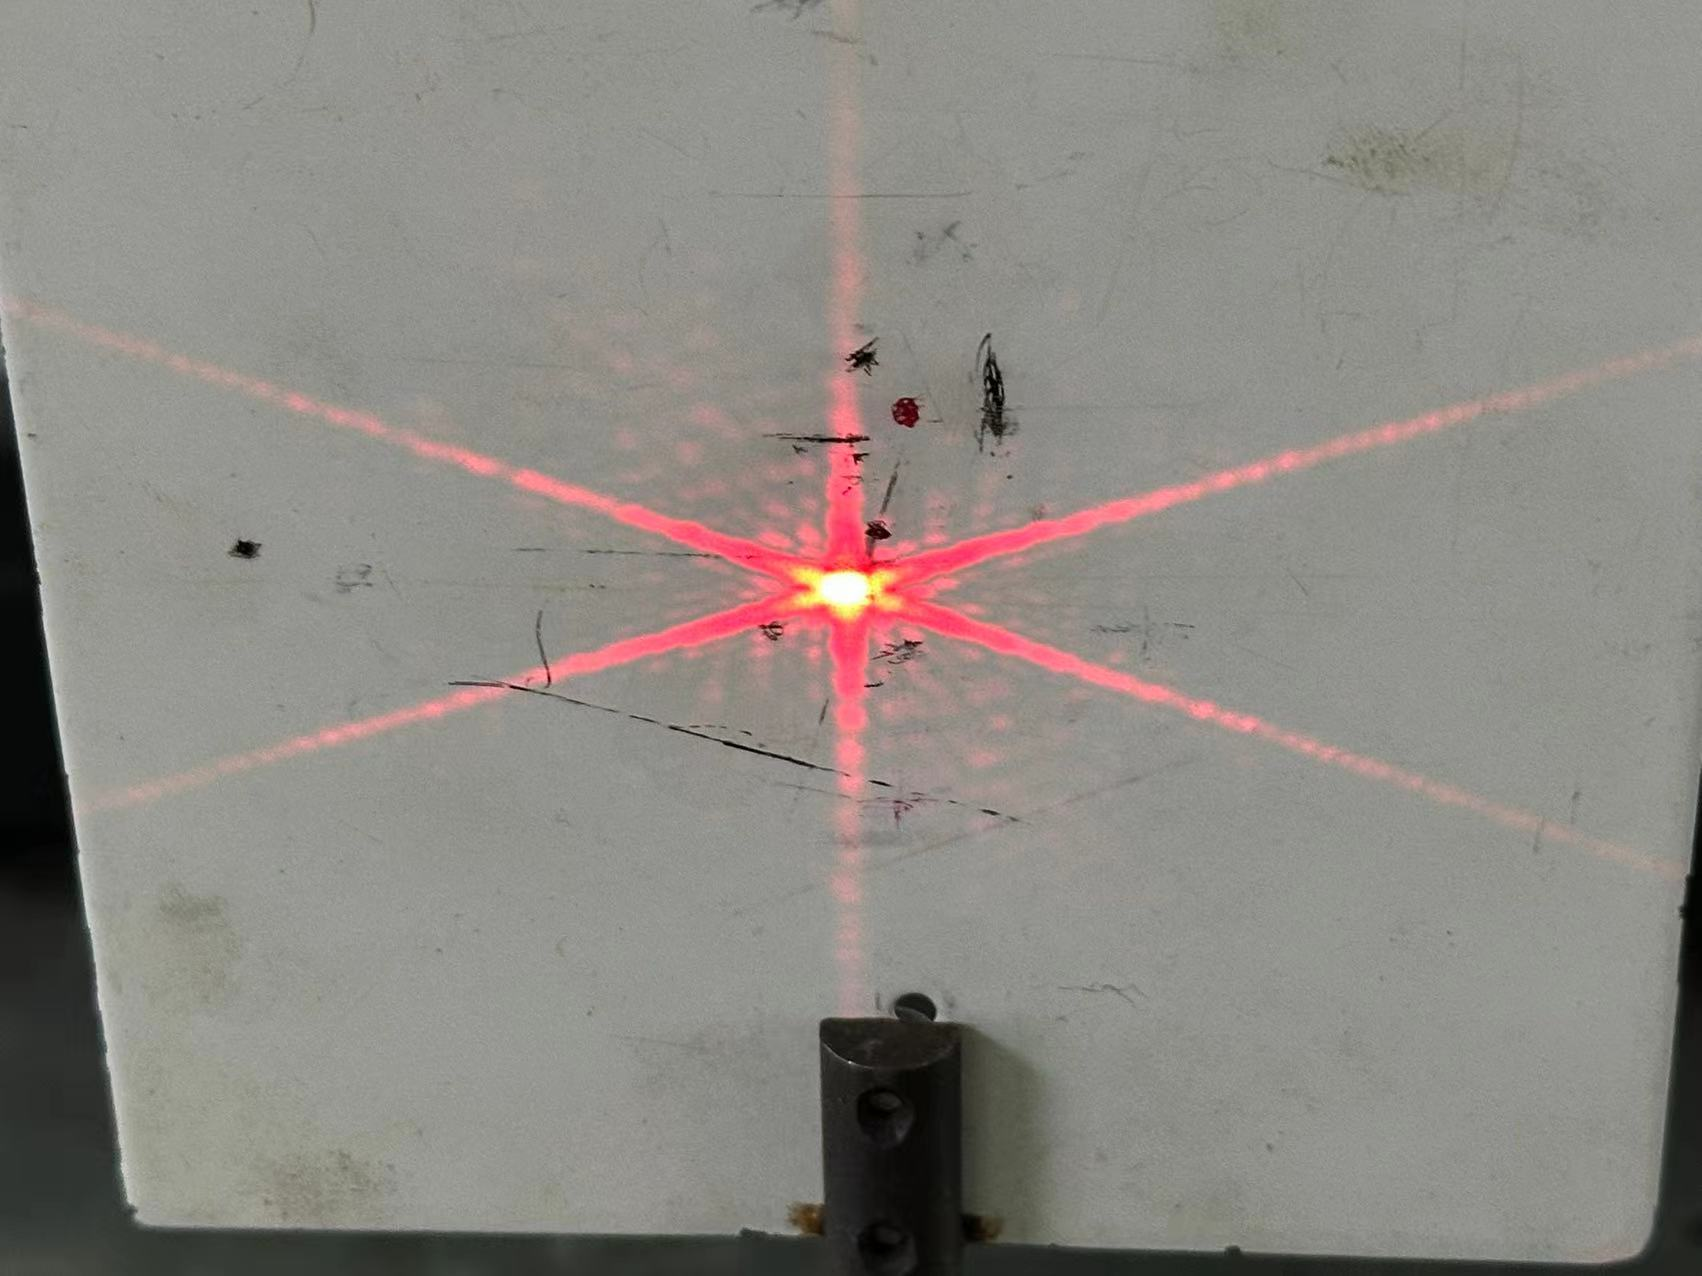
\includegraphics[width=6cm]{0.jpg}
		\caption{等腰三角形衍射图案}
	\end{figure}
	\section{实验记录纸}
	\begin{figure}[H]
		\centering
		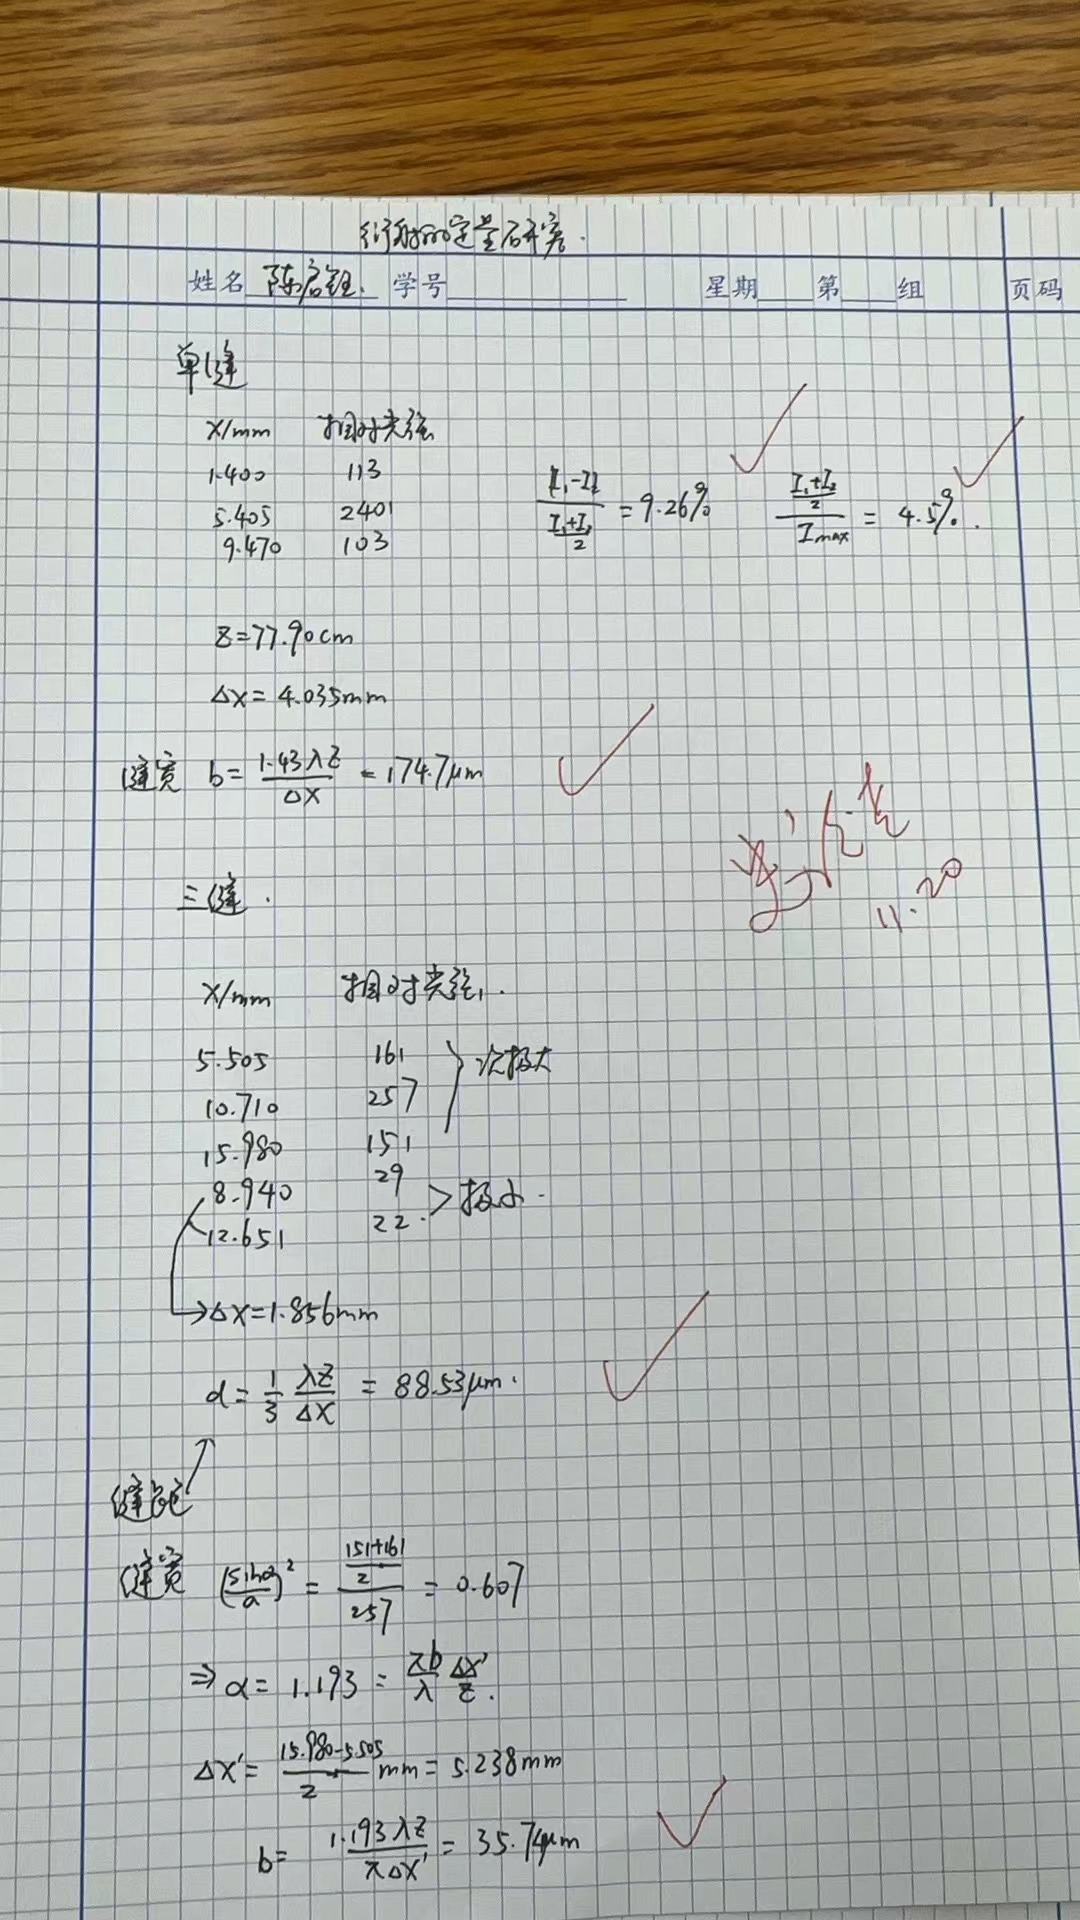
\includegraphics[width=13cm]{note.jpg}
	\end{figure}
\end{document}